% Created by tikzDevice version 0.10.1 on 2017-10-30 17:28:45
% !TEX encoding = UTF-8 Unicode
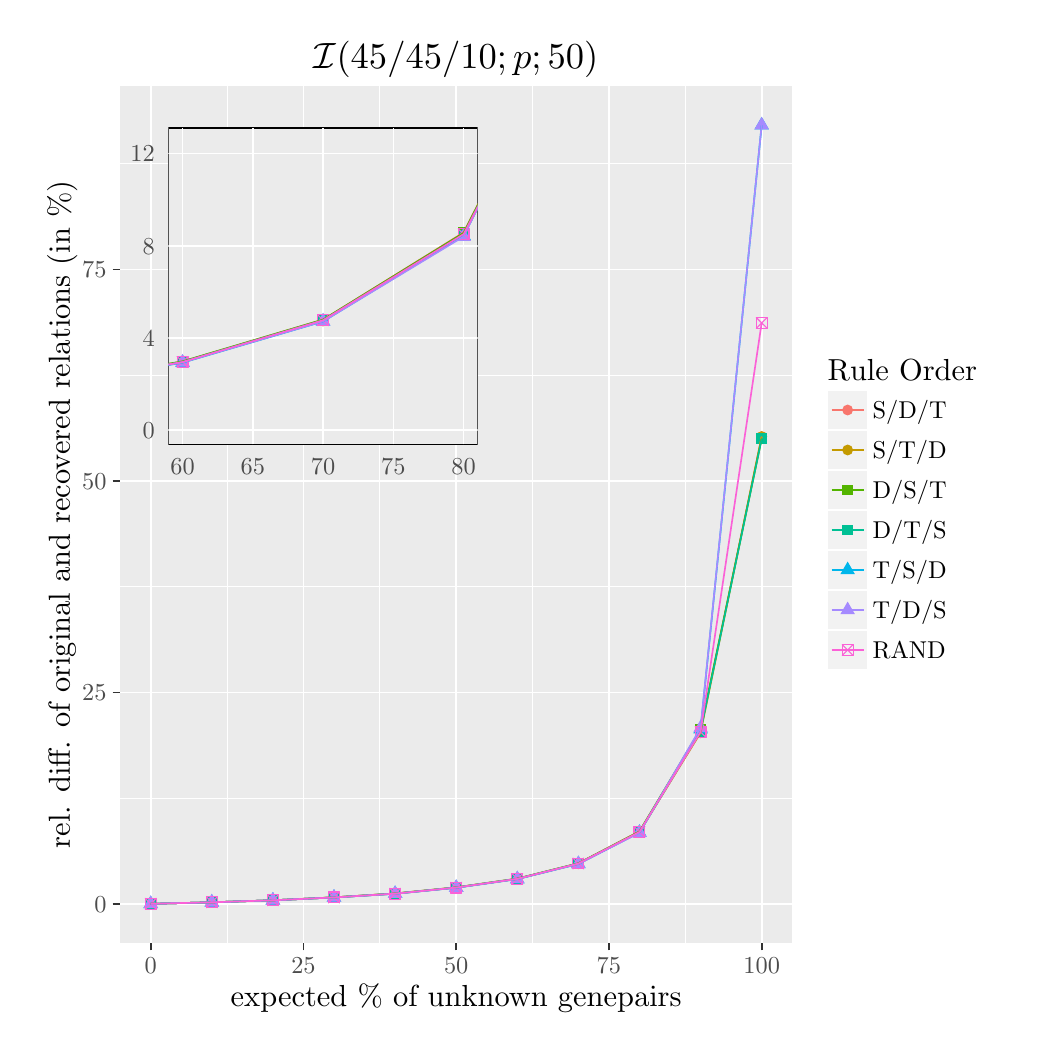
\begin{tikzpicture}[x=1pt,y=1pt]
\definecolor{fillColor}{RGB}{255,255,255}
\path[use as bounding box,fill=fillColor,fill opacity=0.00] (0,0) rectangle (361.35,361.35);
\begin{scope}
\path[clip] (  0.00,  0.00) rectangle (361.35,361.35);
\definecolor{drawColor}{RGB}{255,255,255}
\definecolor{fillColor}{RGB}{255,255,255}

\path[draw=drawColor,line width= 0.6pt,line join=round,line cap=round,fill=fillColor] (  0.00,  0.00) rectangle (361.35,361.35);
\end{scope}
\begin{scope}
\path[clip] ( 33.42, 30.69) rectangle (276.26,340.16);
\definecolor{fillColor}{gray}{0.92}

\path[fill=fillColor] ( 33.42, 30.69) rectangle (276.26,340.16);
\definecolor{drawColor}{RGB}{255,255,255}

\path[draw=drawColor,line width= 0.3pt,line join=round] ( 33.42, 82.95) --
	(276.26, 82.95);

\path[draw=drawColor,line width= 0.3pt,line join=round] ( 33.42,159.36) --
	(276.26,159.36);

\path[draw=drawColor,line width= 0.3pt,line join=round] ( 33.42,235.76) --
	(276.26,235.76);

\path[draw=drawColor,line width= 0.3pt,line join=round] ( 33.42,312.16) --
	(276.26,312.16);

\path[draw=drawColor,line width= 0.3pt,line join=round] ( 72.06, 30.69) --
	( 72.06,340.16);

\path[draw=drawColor,line width= 0.3pt,line join=round] (127.25, 30.69) --
	(127.25,340.16);

\path[draw=drawColor,line width= 0.3pt,line join=round] (182.44, 30.69) --
	(182.44,340.16);

\path[draw=drawColor,line width= 0.3pt,line join=round] (237.63, 30.69) --
	(237.63,340.16);

\path[draw=drawColor,line width= 0.6pt,line join=round] ( 33.42, 44.75) --
	(276.26, 44.75);

\path[draw=drawColor,line width= 0.6pt,line join=round] ( 33.42,121.16) --
	(276.26,121.16);

\path[draw=drawColor,line width= 0.6pt,line join=round] ( 33.42,197.56) --
	(276.26,197.56);

\path[draw=drawColor,line width= 0.6pt,line join=round] ( 33.42,273.96) --
	(276.26,273.96);

\path[draw=drawColor,line width= 0.6pt,line join=round] ( 44.46, 30.69) --
	( 44.46,340.16);

\path[draw=drawColor,line width= 0.6pt,line join=round] ( 99.65, 30.69) --
	( 99.65,340.16);

\path[draw=drawColor,line width= 0.6pt,line join=round] (154.84, 30.69) --
	(154.84,340.16);

\path[draw=drawColor,line width= 0.6pt,line join=round] (210.03, 30.69) --
	(210.03,340.16);

\path[draw=drawColor,line width= 0.6pt,line join=round] (265.23, 30.69) --
	(265.23,340.16);
\definecolor{fillColor}{RGB}{248,118,109}

\path[fill=fillColor] ( 44.46, 44.75) circle (  1.96);

\path[fill=fillColor] ( 66.54, 45.31) circle (  1.96);

\path[fill=fillColor] ( 88.61, 46.03) circle (  1.96);

\path[fill=fillColor] (110.69, 47.09) circle (  1.96);

\path[fill=fillColor] (132.77, 48.50) circle (  1.96);

\path[fill=fillColor] (154.84, 50.69) circle (  1.96);

\path[fill=fillColor] (176.92, 53.83) circle (  1.96);

\path[fill=fillColor] (199.00, 59.39) circle (  1.96);

\path[fill=fillColor] (221.07, 70.96) circle (  1.96);

\path[fill=fillColor] (243.15,107.51) circle (  1.96);

\path[fill=fillColor] (265.23,213.57) circle (  1.96);
\definecolor{fillColor}{RGB}{196,154,0}

\path[fill=fillColor] ( 44.46, 44.75) circle (  1.96);

\path[fill=fillColor] ( 66.54, 45.31) circle (  1.96);

\path[fill=fillColor] ( 88.61, 46.02) circle (  1.96);

\path[fill=fillColor] (110.69, 47.08) circle (  1.96);

\path[fill=fillColor] (132.77, 48.46) circle (  1.96);

\path[fill=fillColor] (154.84, 50.63) circle (  1.96);

\path[fill=fillColor] (176.92, 53.76) circle (  1.96);

\path[fill=fillColor] (199.00, 59.22) circle (  1.96);

\path[fill=fillColor] (221.07, 70.70) circle (  1.96);

\path[fill=fillColor] (243.15,106.57) circle (  1.96);

\path[fill=fillColor] (265.23,213.57) circle (  1.96);
\definecolor{fillColor}{RGB}{83,180,0}

\path[fill=fillColor] ( 42.50, 42.79) --
	( 46.42, 42.79) --
	( 46.42, 46.72) --
	( 42.50, 46.72) --
	cycle;

\path[fill=fillColor] ( 64.58, 43.35) --
	( 68.50, 43.35) --
	( 68.50, 47.27) --
	( 64.58, 47.27) --
	cycle;

\path[fill=fillColor] ( 86.65, 44.08) --
	( 90.58, 44.08) --
	( 90.58, 48.00) --
	( 86.65, 48.00) --
	cycle;

\path[fill=fillColor] (108.73, 45.13) --
	(112.65, 45.13) --
	(112.65, 49.06) --
	(108.73, 49.06) --
	cycle;

\path[fill=fillColor] (130.81, 46.52) --
	(134.73, 46.52) --
	(134.73, 50.44) --
	(130.81, 50.44) --
	cycle;

\path[fill=fillColor] (152.88, 48.74) --
	(156.81, 48.74) --
	(156.81, 52.67) --
	(152.88, 52.67) --
	cycle;

\path[fill=fillColor] (174.96, 51.90) --
	(178.88, 51.90) --
	(178.88, 55.83) --
	(174.96, 55.83) --
	cycle;

\path[fill=fillColor] (197.03, 57.45) --
	(200.96, 57.45) --
	(200.96, 61.37) --
	(197.03, 61.37) --
	cycle;

\path[fill=fillColor] (219.11, 68.94) --
	(223.03, 68.94) --
	(223.03, 72.87) --
	(219.11, 72.87) --
	cycle;

\path[fill=fillColor] (241.19,105.89) --
	(245.11,105.89) --
	(245.11,109.81) --
	(241.19,109.81) --
	cycle;

\path[fill=fillColor] (263.26,210.84) --
	(267.19,210.84) --
	(267.19,214.77) --
	(263.26,214.77) --
	cycle;
\definecolor{fillColor}{RGB}{0,192,148}

\path[fill=fillColor] ( 42.50, 42.79) --
	( 46.42, 42.79) --
	( 46.42, 46.72) --
	( 42.50, 46.72) --
	cycle;

\path[fill=fillColor] ( 64.58, 43.34) --
	( 68.50, 43.34) --
	( 68.50, 47.27) --
	( 64.58, 47.27) --
	cycle;

\path[fill=fillColor] ( 86.65, 44.07) --
	( 90.58, 44.07) --
	( 90.58, 48.00) --
	( 86.65, 48.00) --
	cycle;

\path[fill=fillColor] (108.73, 45.10) --
	(112.65, 45.10) --
	(112.65, 49.02) --
	(108.73, 49.02) --
	cycle;

\path[fill=fillColor] (130.81, 46.46) --
	(134.73, 46.46) --
	(134.73, 50.39) --
	(130.81, 50.39) --
	cycle;

\path[fill=fillColor] (152.88, 48.67) --
	(156.81, 48.67) --
	(156.81, 52.60) --
	(152.88, 52.60) --
	cycle;

\path[fill=fillColor] (174.96, 51.82) --
	(178.88, 51.82) --
	(178.88, 55.74) --
	(174.96, 55.74) --
	cycle;

\path[fill=fillColor] (197.03, 57.34) --
	(200.96, 57.34) --
	(200.96, 61.27) --
	(197.03, 61.27) --
	cycle;

\path[fill=fillColor] (219.11, 68.61) --
	(223.03, 68.61) --
	(223.03, 72.54) --
	(219.11, 72.54) --
	cycle;

\path[fill=fillColor] (241.19,105.18) --
	(245.11,105.18) --
	(245.11,109.11) --
	(241.19,109.11) --
	cycle;

\path[fill=fillColor] (263.26,210.84) --
	(267.19,210.84) --
	(267.19,214.77) --
	(263.26,214.77) --
	cycle;
\definecolor{fillColor}{RGB}{0,182,235}

\path[fill=fillColor] ( 44.46, 47.80) --
	( 47.10, 43.23) --
	( 41.82, 43.23) --
	cycle;

\path[fill=fillColor] ( 66.54, 48.35) --
	( 69.18, 43.77) --
	( 63.90, 43.77) --
	cycle;

\path[fill=fillColor] ( 88.61, 49.07) --
	( 91.26, 44.50) --
	( 85.97, 44.50) --
	cycle;

\path[fill=fillColor] (110.69, 50.10) --
	(113.33, 45.52) --
	(108.05, 45.52) --
	cycle;

\path[fill=fillColor] (132.77, 51.46) --
	(135.41, 46.88) --
	(130.12, 46.88) --
	cycle;

\path[fill=fillColor] (154.84, 53.62) --
	(157.49, 49.04) --
	(152.20, 49.04) --
	cycle;

\path[fill=fillColor] (176.92, 56.74) --
	(179.56, 52.16) --
	(174.28, 52.16) --
	cycle;

\path[fill=fillColor] (199.00, 62.21) --
	(201.64, 57.64) --
	(196.35, 57.64) --
	cycle;

\path[fill=fillColor] (221.07, 73.58) --
	(223.72, 69.00) --
	(218.43, 69.00) --
	cycle;

\path[fill=fillColor] (243.15,110.94) --
	(245.79,106.37) --
	(240.51,106.37) --
	cycle;

\path[fill=fillColor] (265.23,329.14) --
	(267.87,324.57) --
	(262.58,324.57) --
	cycle;
\definecolor{fillColor}{RGB}{165,138,255}

\path[fill=fillColor] ( 44.46, 47.80) --
	( 47.10, 43.23) --
	( 41.82, 43.23) --
	cycle;

\path[fill=fillColor] ( 66.54, 48.35) --
	( 69.18, 43.78) --
	( 63.90, 43.78) --
	cycle;

\path[fill=fillColor] ( 88.61, 49.08) --
	( 91.26, 44.50) --
	( 85.97, 44.50) --
	cycle;

\path[fill=fillColor] (110.69, 50.10) --
	(113.33, 45.53) --
	(108.05, 45.53) --
	cycle;

\path[fill=fillColor] (132.77, 51.44) --
	(135.41, 46.87) --
	(130.12, 46.87) --
	cycle;

\path[fill=fillColor] (154.84, 53.64) --
	(157.49, 49.07) --
	(152.20, 49.07) --
	cycle;

\path[fill=fillColor] (176.92, 56.77) --
	(179.56, 52.20) --
	(174.28, 52.20) --
	cycle;

\path[fill=fillColor] (199.00, 62.22) --
	(201.64, 57.64) --
	(196.35, 57.64) --
	cycle;

\path[fill=fillColor] (221.07, 73.47) --
	(223.72, 68.90) --
	(218.43, 68.90) --
	cycle;

\path[fill=fillColor] (243.15,111.35) --
	(245.79,106.77) --
	(240.51,106.77) --
	cycle;

\path[fill=fillColor] (265.23,329.14) --
	(267.87,324.57) --
	(262.58,324.57) --
	cycle;
\definecolor{drawColor}{RGB}{251,97,215}

\path[draw=drawColor,line width= 0.4pt,line join=round,line cap=round] ( 42.50, 42.79) rectangle ( 46.42, 46.72);

\path[draw=drawColor,line width= 0.4pt,line join=round,line cap=round] ( 42.50, 42.79) -- ( 46.42, 46.72);

\path[draw=drawColor,line width= 0.4pt,line join=round,line cap=round] ( 42.50, 46.72) -- ( 46.42, 42.79);

\path[draw=drawColor,line width= 0.4pt,line join=round,line cap=round] ( 64.58, 43.35) rectangle ( 68.50, 47.27);

\path[draw=drawColor,line width= 0.4pt,line join=round,line cap=round] ( 64.58, 43.35) -- ( 68.50, 47.27);

\path[draw=drawColor,line width= 0.4pt,line join=round,line cap=round] ( 64.58, 47.27) -- ( 68.50, 43.35);

\path[draw=drawColor,line width= 0.4pt,line join=round,line cap=round] ( 86.65, 44.07) rectangle ( 90.58, 47.99);

\path[draw=drawColor,line width= 0.4pt,line join=round,line cap=round] ( 86.65, 44.07) -- ( 90.58, 47.99);

\path[draw=drawColor,line width= 0.4pt,line join=round,line cap=round] ( 86.65, 47.99) -- ( 90.58, 44.07);

\path[draw=drawColor,line width= 0.4pt,line join=round,line cap=round] (108.73, 45.10) rectangle (112.65, 49.02);

\path[draw=drawColor,line width= 0.4pt,line join=round,line cap=round] (108.73, 45.10) -- (112.65, 49.02);

\path[draw=drawColor,line width= 0.4pt,line join=round,line cap=round] (108.73, 49.02) -- (112.65, 45.10);

\path[draw=drawColor,line width= 0.4pt,line join=round,line cap=round] (130.81, 46.47) rectangle (134.73, 50.40);

\path[draw=drawColor,line width= 0.4pt,line join=round,line cap=round] (130.81, 46.47) -- (134.73, 50.40);

\path[draw=drawColor,line width= 0.4pt,line join=round,line cap=round] (130.81, 50.40) -- (134.73, 46.47);

\path[draw=drawColor,line width= 0.4pt,line join=round,line cap=round] (152.88, 48.65) rectangle (156.81, 52.58);

\path[draw=drawColor,line width= 0.4pt,line join=round,line cap=round] (152.88, 48.65) -- (156.81, 52.58);

\path[draw=drawColor,line width= 0.4pt,line join=round,line cap=round] (152.88, 52.58) -- (156.81, 48.65);

\path[draw=drawColor,line width= 0.4pt,line join=round,line cap=round] (174.96, 51.82) rectangle (178.88, 55.74);

\path[draw=drawColor,line width= 0.4pt,line join=round,line cap=round] (174.96, 51.82) -- (178.88, 55.74);

\path[draw=drawColor,line width= 0.4pt,line join=round,line cap=round] (174.96, 55.74) -- (178.88, 51.82);

\path[draw=drawColor,line width= 0.4pt,line join=round,line cap=round] (197.03, 57.36) rectangle (200.96, 61.28);

\path[draw=drawColor,line width= 0.4pt,line join=round,line cap=round] (197.03, 57.36) -- (200.96, 61.28);

\path[draw=drawColor,line width= 0.4pt,line join=round,line cap=round] (197.03, 61.28) -- (200.96, 57.36);

\path[draw=drawColor,line width= 0.4pt,line join=round,line cap=round] (219.11, 68.78) rectangle (223.03, 72.70);

\path[draw=drawColor,line width= 0.4pt,line join=round,line cap=round] (219.11, 68.78) -- (223.03, 72.70);

\path[draw=drawColor,line width= 0.4pt,line join=round,line cap=round] (219.11, 72.70) -- (223.03, 68.78);

\path[draw=drawColor,line width= 0.4pt,line join=round,line cap=round] (241.19,104.89) rectangle (245.11,108.81);

\path[draw=drawColor,line width= 0.4pt,line join=round,line cap=round] (241.19,104.89) -- (245.11,108.81);

\path[draw=drawColor,line width= 0.4pt,line join=round,line cap=round] (241.19,108.81) -- (245.11,104.89);

\path[draw=drawColor,line width= 0.4pt,line join=round,line cap=round] (263.26,252.71) rectangle (267.19,256.63);

\path[draw=drawColor,line width= 0.4pt,line join=round,line cap=round] (263.26,252.71) -- (267.19,256.63);

\path[draw=drawColor,line width= 0.4pt,line join=round,line cap=round] (263.26,256.63) -- (267.19,252.71);
\definecolor{drawColor}{RGB}{248,118,109}

\path[draw=drawColor,line width= 0.6pt,line join=round] ( 44.46, 44.75) --
	( 66.54, 45.31) --
	( 88.61, 46.03) --
	(110.69, 47.09) --
	(132.77, 48.50) --
	(154.84, 50.69) --
	(176.92, 53.83) --
	(199.00, 59.39) --
	(221.07, 70.96) --
	(243.15,107.51) --
	(265.23,213.57);
\definecolor{drawColor}{RGB}{196,154,0}

\path[draw=drawColor,line width= 0.6pt,line join=round] ( 44.46, 44.75) --
	( 66.54, 45.31) --
	( 88.61, 46.02) --
	(110.69, 47.08) --
	(132.77, 48.46) --
	(154.84, 50.63) --
	(176.92, 53.76) --
	(199.00, 59.22) --
	(221.07, 70.70) --
	(243.15,106.57) --
	(265.23,213.57);
\definecolor{drawColor}{RGB}{83,180,0}

\path[draw=drawColor,line width= 0.6pt,line join=round] ( 44.46, 44.75) --
	( 66.54, 45.31) --
	( 88.61, 46.04) --
	(110.69, 47.10) --
	(132.77, 48.48) --
	(154.84, 50.70) --
	(176.92, 53.87) --
	(199.00, 59.41) --
	(221.07, 70.91) --
	(243.15,107.85) --
	(265.23,212.81);
\definecolor{drawColor}{RGB}{0,192,148}

\path[draw=drawColor,line width= 0.6pt,line join=round] ( 44.46, 44.75) --
	( 66.54, 45.31) --
	( 88.61, 46.04) --
	(110.69, 47.06) --
	(132.77, 48.43) --
	(154.84, 50.63) --
	(176.92, 53.78) --
	(199.00, 59.30) --
	(221.07, 70.57) --
	(243.15,107.14) --
	(265.23,212.81);
\definecolor{drawColor}{RGB}{0,182,235}

\path[draw=drawColor,line width= 0.6pt,line join=round] ( 44.46, 44.75) --
	( 66.54, 45.30) --
	( 88.61, 46.02) --
	(110.69, 47.05) --
	(132.77, 48.41) --
	(154.84, 50.56) --
	(176.92, 53.69) --
	(199.00, 59.16) --
	(221.07, 70.53) --
	(243.15,107.89) --
	(265.23,326.09);
\definecolor{drawColor}{RGB}{165,138,255}

\path[draw=drawColor,line width= 0.6pt,line join=round] ( 44.46, 44.75) --
	( 66.54, 45.30) --
	( 88.61, 46.03) --
	(110.69, 47.05) --
	(132.77, 48.39) --
	(154.84, 50.59) --
	(176.92, 53.72) --
	(199.00, 59.17) --
	(221.07, 70.42) --
	(243.15,108.30) --
	(265.23,326.09);
\definecolor{drawColor}{RGB}{251,97,215}

\path[draw=drawColor,line width= 0.6pt,line join=round] ( 44.46, 44.75) --
	( 66.54, 45.31) --
	( 88.61, 46.03) --
	(110.69, 47.06) --
	(132.77, 48.43) --
	(154.84, 50.62) --
	(176.92, 53.78) --
	(199.00, 59.32) --
	(221.07, 70.74) --
	(243.15,106.85) --
	(265.23,254.67);
\end{scope}
\begin{scope}
\path[clip] (  0.00,  0.00) rectangle (361.35,361.35);
\definecolor{drawColor}{gray}{0.30}

\node[text=drawColor,anchor=base east,inner sep=0pt, outer sep=0pt, scale=  0.88] at ( 28.47, 41.72) {0};

\node[text=drawColor,anchor=base east,inner sep=0pt, outer sep=0pt, scale=  0.88] at ( 28.47,118.13) {25};

\node[text=drawColor,anchor=base east,inner sep=0pt, outer sep=0pt, scale=  0.88] at ( 28.47,194.53) {50};

\node[text=drawColor,anchor=base east,inner sep=0pt, outer sep=0pt, scale=  0.88] at ( 28.47,270.93) {75};
\end{scope}
\begin{scope}
\path[clip] (  0.00,  0.00) rectangle (361.35,361.35);
\definecolor{drawColor}{gray}{0.20}

\path[draw=drawColor,line width= 0.6pt,line join=round] ( 30.67, 44.75) --
	( 33.42, 44.75);

\path[draw=drawColor,line width= 0.6pt,line join=round] ( 30.67,121.16) --
	( 33.42,121.16);

\path[draw=drawColor,line width= 0.6pt,line join=round] ( 30.67,197.56) --
	( 33.42,197.56);

\path[draw=drawColor,line width= 0.6pt,line join=round] ( 30.67,273.96) --
	( 33.42,273.96);
\end{scope}
\begin{scope}
\path[clip] (  0.00,  0.00) rectangle (361.35,361.35);
\definecolor{drawColor}{gray}{0.20}

\path[draw=drawColor,line width= 0.6pt,line join=round] ( 44.46, 27.94) --
	( 44.46, 30.69);

\path[draw=drawColor,line width= 0.6pt,line join=round] ( 99.65, 27.94) --
	( 99.65, 30.69);

\path[draw=drawColor,line width= 0.6pt,line join=round] (154.84, 27.94) --
	(154.84, 30.69);

\path[draw=drawColor,line width= 0.6pt,line join=round] (210.03, 27.94) --
	(210.03, 30.69);

\path[draw=drawColor,line width= 0.6pt,line join=round] (265.23, 27.94) --
	(265.23, 30.69);
\end{scope}
\begin{scope}
\path[clip] (  0.00,  0.00) rectangle (361.35,361.35);
\definecolor{drawColor}{gray}{0.30}

\node[text=drawColor,anchor=base,inner sep=0pt, outer sep=0pt, scale=  0.88] at ( 44.46, 19.68) {0};

\node[text=drawColor,anchor=base,inner sep=0pt, outer sep=0pt, scale=  0.88] at ( 99.65, 19.68) {25};

\node[text=drawColor,anchor=base,inner sep=0pt, outer sep=0pt, scale=  0.88] at (154.84, 19.68) {50};

\node[text=drawColor,anchor=base,inner sep=0pt, outer sep=0pt, scale=  0.88] at (210.03, 19.68) {75};

\node[text=drawColor,anchor=base,inner sep=0pt, outer sep=0pt, scale=  0.88] at (265.23, 19.68) {100};
\end{scope}
\begin{scope}
\path[clip] (  0.00,  0.00) rectangle (361.35,361.35);
\definecolor{drawColor}{RGB}{0,0,0}

\node[text=drawColor,anchor=base,inner sep=0pt, outer sep=0pt, scale=  1.10] at (154.84,  7.70) {expected \% of unknown genepairs};
\end{scope}
\begin{scope}
\path[clip] (  0.00,  0.00) rectangle (361.35,361.35);
\definecolor{drawColor}{RGB}{0,0,0}

\node[text=drawColor,rotate= 90.00,anchor=base,inner sep=0pt, outer sep=0pt, scale=  1.10] at ( 15.28,185.42) {rel. diff. of original and recovered relations (in \%)};
\end{scope}
\begin{scope}
\path[clip] (  0.00,  0.00) rectangle (361.35,361.35);
\definecolor{fillColor}{RGB}{255,255,255}

\path[fill=fillColor] (284.80,124.97) rectangle (347.31,245.87);
\end{scope}
\begin{scope}
\path[clip] (  0.00,  0.00) rectangle (361.35,361.35);
\definecolor{drawColor}{RGB}{0,0,0}

\node[text=drawColor,anchor=base west,inner sep=0pt, outer sep=0pt, scale=  1.10] at (289.07,234.03) {Rule Order};
\end{scope}
\begin{scope}
\path[clip] (  0.00,  0.00) rectangle (361.35,361.35);
\definecolor{drawColor}{RGB}{255,255,255}
\definecolor{fillColor}{gray}{0.95}

\path[draw=drawColor,line width= 0.6pt,line join=round,line cap=round,fill=fillColor] (289.07,215.96) rectangle (303.52,230.42);
\end{scope}
\begin{scope}
\path[clip] (  0.00,  0.00) rectangle (361.35,361.35);
\definecolor{fillColor}{RGB}{248,118,109}

\path[fill=fillColor] (296.29,223.19) circle (  1.96);
\end{scope}
\begin{scope}
\path[clip] (  0.00,  0.00) rectangle (361.35,361.35);
\definecolor{drawColor}{RGB}{248,118,109}

\path[draw=drawColor,line width= 0.6pt,line join=round] (290.51,223.19) -- (302.08,223.19);
\end{scope}
\begin{scope}
\path[clip] (  0.00,  0.00) rectangle (361.35,361.35);
\definecolor{drawColor}{RGB}{255,255,255}
\definecolor{fillColor}{gray}{0.95}

\path[draw=drawColor,line width= 0.6pt,line join=round,line cap=round,fill=fillColor] (289.07,201.51) rectangle (303.52,215.96);
\end{scope}
\begin{scope}
\path[clip] (  0.00,  0.00) rectangle (361.35,361.35);
\definecolor{fillColor}{RGB}{196,154,0}

\path[fill=fillColor] (296.29,208.74) circle (  1.96);
\end{scope}
\begin{scope}
\path[clip] (  0.00,  0.00) rectangle (361.35,361.35);
\definecolor{drawColor}{RGB}{196,154,0}

\path[draw=drawColor,line width= 0.6pt,line join=round] (290.51,208.74) -- (302.08,208.74);
\end{scope}
\begin{scope}
\path[clip] (  0.00,  0.00) rectangle (361.35,361.35);
\definecolor{drawColor}{RGB}{255,255,255}
\definecolor{fillColor}{gray}{0.95}

\path[draw=drawColor,line width= 0.6pt,line join=round,line cap=round,fill=fillColor] (289.07,187.06) rectangle (303.52,201.51);
\end{scope}
\begin{scope}
\path[clip] (  0.00,  0.00) rectangle (361.35,361.35);
\definecolor{fillColor}{RGB}{83,180,0}

\path[fill=fillColor] (294.33,192.32) --
	(298.26,192.32) --
	(298.26,196.24) --
	(294.33,196.24) --
	cycle;
\end{scope}
\begin{scope}
\path[clip] (  0.00,  0.00) rectangle (361.35,361.35);
\definecolor{drawColor}{RGB}{83,180,0}

\path[draw=drawColor,line width= 0.6pt,line join=round] (290.51,194.28) -- (302.08,194.28);
\end{scope}
\begin{scope}
\path[clip] (  0.00,  0.00) rectangle (361.35,361.35);
\definecolor{drawColor}{RGB}{255,255,255}
\definecolor{fillColor}{gray}{0.95}

\path[draw=drawColor,line width= 0.6pt,line join=round,line cap=round,fill=fillColor] (289.07,172.60) rectangle (303.52,187.06);
\end{scope}
\begin{scope}
\path[clip] (  0.00,  0.00) rectangle (361.35,361.35);
\definecolor{fillColor}{RGB}{0,192,148}

\path[fill=fillColor] (294.33,177.87) --
	(298.26,177.87) --
	(298.26,181.79) --
	(294.33,181.79) --
	cycle;
\end{scope}
\begin{scope}
\path[clip] (  0.00,  0.00) rectangle (361.35,361.35);
\definecolor{drawColor}{RGB}{0,192,148}

\path[draw=drawColor,line width= 0.6pt,line join=round] (290.51,179.83) -- (302.08,179.83);
\end{scope}
\begin{scope}
\path[clip] (  0.00,  0.00) rectangle (361.35,361.35);
\definecolor{drawColor}{RGB}{255,255,255}
\definecolor{fillColor}{gray}{0.95}

\path[draw=drawColor,line width= 0.6pt,line join=round,line cap=round,fill=fillColor] (289.07,158.15) rectangle (303.52,172.60);
\end{scope}
\begin{scope}
\path[clip] (  0.00,  0.00) rectangle (361.35,361.35);
\definecolor{fillColor}{RGB}{0,182,235}

\path[fill=fillColor] (296.29,168.43) --
	(298.94,163.85) --
	(293.65,163.85) --
	cycle;
\end{scope}
\begin{scope}
\path[clip] (  0.00,  0.00) rectangle (361.35,361.35);
\definecolor{drawColor}{RGB}{0,182,235}

\path[draw=drawColor,line width= 0.6pt,line join=round] (290.51,165.37) -- (302.08,165.37);
\end{scope}
\begin{scope}
\path[clip] (  0.00,  0.00) rectangle (361.35,361.35);
\definecolor{drawColor}{RGB}{255,255,255}
\definecolor{fillColor}{gray}{0.95}

\path[draw=drawColor,line width= 0.6pt,line join=round,line cap=round,fill=fillColor] (289.07,143.69) rectangle (303.52,158.15);
\end{scope}
\begin{scope}
\path[clip] (  0.00,  0.00) rectangle (361.35,361.35);
\definecolor{fillColor}{RGB}{165,138,255}

\path[fill=fillColor] (296.29,153.97) --
	(298.94,149.39) --
	(293.65,149.39) --
	cycle;
\end{scope}
\begin{scope}
\path[clip] (  0.00,  0.00) rectangle (361.35,361.35);
\definecolor{drawColor}{RGB}{165,138,255}

\path[draw=drawColor,line width= 0.6pt,line join=round] (290.51,150.92) -- (302.08,150.92);
\end{scope}
\begin{scope}
\path[clip] (  0.00,  0.00) rectangle (361.35,361.35);
\definecolor{drawColor}{RGB}{255,255,255}
\definecolor{fillColor}{gray}{0.95}

\path[draw=drawColor,line width= 0.6pt,line join=round,line cap=round,fill=fillColor] (289.07,129.24) rectangle (303.52,143.69);
\end{scope}
\begin{scope}
\path[clip] (  0.00,  0.00) rectangle (361.35,361.35);
\definecolor{drawColor}{RGB}{251,97,215}

\path[draw=drawColor,line width= 0.4pt,line join=round,line cap=round] (294.33,134.50) rectangle (298.26,138.43);

\path[draw=drawColor,line width= 0.4pt,line join=round,line cap=round] (294.33,134.50) -- (298.26,138.43);

\path[draw=drawColor,line width= 0.4pt,line join=round,line cap=round] (294.33,138.43) -- (298.26,134.50);
\end{scope}
\begin{scope}
\path[clip] (  0.00,  0.00) rectangle (361.35,361.35);
\definecolor{drawColor}{RGB}{251,97,215}

\path[draw=drawColor,line width= 0.6pt,line join=round] (290.51,136.47) -- (302.08,136.47);
\end{scope}
\begin{scope}
\path[clip] (  0.00,  0.00) rectangle (361.35,361.35);
\definecolor{drawColor}{RGB}{0,0,0}

\node[text=drawColor,anchor=base west,inner sep=0pt, outer sep=0pt, scale=  0.88] at (305.33,220.16) {S/D/T};
\end{scope}
\begin{scope}
\path[clip] (  0.00,  0.00) rectangle (361.35,361.35);
\definecolor{drawColor}{RGB}{0,0,0}

\node[text=drawColor,anchor=base west,inner sep=0pt, outer sep=0pt, scale=  0.88] at (305.33,205.71) {S/T/D};
\end{scope}
\begin{scope}
\path[clip] (  0.00,  0.00) rectangle (361.35,361.35);
\definecolor{drawColor}{RGB}{0,0,0}

\node[text=drawColor,anchor=base west,inner sep=0pt, outer sep=0pt, scale=  0.88] at (305.33,191.25) {D/S/T};
\end{scope}
\begin{scope}
\path[clip] (  0.00,  0.00) rectangle (361.35,361.35);
\definecolor{drawColor}{RGB}{0,0,0}

\node[text=drawColor,anchor=base west,inner sep=0pt, outer sep=0pt, scale=  0.88] at (305.33,176.80) {D/T/S};
\end{scope}
\begin{scope}
\path[clip] (  0.00,  0.00) rectangle (361.35,361.35);
\definecolor{drawColor}{RGB}{0,0,0}

\node[text=drawColor,anchor=base west,inner sep=0pt, outer sep=0pt, scale=  0.88] at (305.33,162.34) {T/S/D};
\end{scope}
\begin{scope}
\path[clip] (  0.00,  0.00) rectangle (361.35,361.35);
\definecolor{drawColor}{RGB}{0,0,0}

\node[text=drawColor,anchor=base west,inner sep=0pt, outer sep=0pt, scale=  0.88] at (305.33,147.89) {T/D/S};
\end{scope}
\begin{scope}
\path[clip] (  0.00,  0.00) rectangle (361.35,361.35);
\definecolor{drawColor}{RGB}{0,0,0}

\node[text=drawColor,anchor=base west,inner sep=0pt, outer sep=0pt, scale=  0.88] at (305.33,133.44) {RAND};
\end{scope}
\begin{scope}
\path[clip] (  0.00,  0.00) rectangle (361.35,361.35);
\definecolor{drawColor}{RGB}{0,0,0}

\node[text=drawColor,anchor=base,inner sep=0pt, outer sep=0pt, scale=  1.32] at (154.84,346.76) {$\mathcal{I}(45/45/10;p;50)$};
\end{scope}
\begin{scope}
\path[clip] ( 54.20,216.81) rectangle (162.61,325.21);
\definecolor{drawColor}{RGB}{255,255,255}
\definecolor{fillColor}{RGB}{255,255,255}

\path[draw=drawColor,line width= 0.6pt,line join=round,line cap=round,fill=fillColor] ( 54.20,216.81) rectangle (162.61,325.21);
\end{scope}
\begin{scope}
\path[clip] ( 50.88,210.75) rectangle (162.61,325.21);
\definecolor{drawColor}{RGB}{0,0,0}
\definecolor{fillColor}{gray}{0.92}

\path[draw=drawColor,line width= 0.6pt,line join=round,line cap=round,fill=fillColor] ( 50.88,210.75) rectangle (162.61,325.21);
\definecolor{drawColor}{RGB}{255,255,255}

\path[draw=drawColor,line width= 0.6pt,line join=round] ( 50.88,215.95) --
	(162.61,215.95);

\path[draw=drawColor,line width= 0.6pt,line join=round] ( 50.88,249.25) --
	(162.61,249.25);

\path[draw=drawColor,line width= 0.6pt,line join=round] ( 50.88,282.55) --
	(162.61,282.55);

\path[draw=drawColor,line width= 0.6pt,line join=round] ( 50.88,315.85) --
	(162.61,315.85);

\path[draw=drawColor,line width= 0.6pt,line join=round] ( 55.96,210.75) --
	( 55.96,325.21);

\path[draw=drawColor,line width= 0.6pt,line join=round] ( 81.35,210.75) --
	( 81.35,325.21);

\path[draw=drawColor,line width= 0.6pt,line join=round] (106.74,210.75) --
	(106.74,325.21);

\path[draw=drawColor,line width= 0.6pt,line join=round] (132.14,210.75) --
	(132.14,325.21);

\path[draw=drawColor,line width= 0.6pt,line join=round] (157.53,210.75) --
	(157.53,325.21);
\definecolor{fillColor}{RGB}{248,118,109}

\path[fill=fillColor] (  5.17,232.12) circle (  1.96);

\path[fill=fillColor] ( 55.96,240.68) circle (  1.96);

\path[fill=fillColor] (106.74,255.83) circle (  1.96);

\path[fill=fillColor] (157.53,287.34) circle (  1.96);
\definecolor{fillColor}{RGB}{196,154,0}

\path[fill=fillColor] (  5.17,231.95) circle (  1.96);

\path[fill=fillColor] ( 55.96,240.48) circle (  1.96);

\path[fill=fillColor] (106.74,255.36) circle (  1.96);

\path[fill=fillColor] (157.53,286.64) circle (  1.96);
\definecolor{fillColor}{RGB}{83,180,0}

\path[fill=fillColor] (  3.21,230.20) --
	(  7.13,230.20) --
	(  7.13,234.12) --
	(  3.21,234.12) --
	cycle;

\path[fill=fillColor] ( 54.00,238.81) --
	( 57.92,238.81) --
	( 57.92,242.74) --
	( 54.00,242.74) --
	cycle;

\path[fill=fillColor] (104.78,253.91) --
	(108.71,253.91) --
	(108.71,257.83) --
	(104.78,257.83) --
	cycle;

\path[fill=fillColor] (155.57,285.23) --
	(159.49,285.23) --
	(159.49,289.15) --
	(155.57,289.15) --
	cycle;
\definecolor{fillColor}{RGB}{0,192,148}

\path[fill=fillColor] (  3.21,230.01) --
	(  7.13,230.01) --
	(  7.13,233.93) --
	(  3.21,233.93) --
	cycle;

\path[fill=fillColor] ( 54.00,238.57) --
	( 57.92,238.57) --
	( 57.92,242.50) --
	( 54.00,242.50) --
	cycle;

\path[fill=fillColor] (104.78,253.62) --
	(108.71,253.62) --
	(108.71,257.55) --
	(104.78,257.55) --
	cycle;

\path[fill=fillColor] (155.57,284.32) --
	(159.49,284.32) --
	(159.49,288.25) --
	(155.57,288.25) --
	cycle;
\definecolor{fillColor}{RGB}{0,182,235}

\path[fill=fillColor] (  5.17,234.83) --
	(  7.81,230.26) --
	(  2.53,230.26) --
	cycle;

\path[fill=fillColor] ( 55.96,243.35) --
	( 58.60,238.77) --
	( 53.31,238.77) --
	cycle;

\path[fill=fillColor] (106.74,258.25) --
	(109.39,253.67) --
	(104.10,253.67) --
	cycle;

\path[fill=fillColor] (157.53,289.21) --
	(160.17,284.63) --
	(154.89,284.63) --
	cycle;
\definecolor{fillColor}{RGB}{165,138,255}

\path[fill=fillColor] (  5.17,234.91) --
	(  7.81,230.33) --
	(  2.53,230.33) --
	cycle;

\path[fill=fillColor] ( 55.96,243.43) --
	( 58.60,238.86) --
	( 53.31,238.86) --
	cycle;

\path[fill=fillColor] (106.74,258.27) --
	(109.39,253.69) --
	(104.10,253.69) --
	cycle;

\path[fill=fillColor] (157.53,288.92) --
	(160.17,284.35) --
	(154.89,284.35) --
	cycle;
\definecolor{drawColor}{RGB}{251,97,215}

\path[draw=drawColor,line width= 0.4pt,line join=round,line cap=round] (  3.21,229.96) rectangle (  7.13,233.88);

\path[draw=drawColor,line width= 0.4pt,line join=round,line cap=round] (  3.21,229.96) -- (  7.13,233.88);

\path[draw=drawColor,line width= 0.4pt,line join=round,line cap=round] (  3.21,233.88) -- (  7.13,229.96);

\path[draw=drawColor,line width= 0.4pt,line join=round,line cap=round] ( 54.00,238.57) rectangle ( 57.92,242.50);

\path[draw=drawColor,line width= 0.4pt,line join=round,line cap=round] ( 54.00,238.57) -- ( 57.92,242.50);

\path[draw=drawColor,line width= 0.4pt,line join=round,line cap=round] ( 54.00,242.50) -- ( 57.92,238.57);

\path[draw=drawColor,line width= 0.4pt,line join=round,line cap=round] (104.78,253.67) rectangle (108.71,257.60);

\path[draw=drawColor,line width= 0.4pt,line join=round,line cap=round] (104.78,253.67) -- (108.71,257.60);

\path[draw=drawColor,line width= 0.4pt,line join=round,line cap=round] (104.78,257.60) -- (108.71,253.67);

\path[draw=drawColor,line width= 0.4pt,line join=round,line cap=round] (155.57,284.77) rectangle (159.49,288.69);

\path[draw=drawColor,line width= 0.4pt,line join=round,line cap=round] (155.57,284.77) -- (159.49,288.69);

\path[draw=drawColor,line width= 0.4pt,line join=round,line cap=round] (155.57,288.69) -- (159.49,284.77);
\definecolor{drawColor}{RGB}{248,118,109}

\path[draw=drawColor,line width= 0.6pt,line join=round] (  0.00,231.51) --
	(  5.17,232.12) --
	( 55.96,240.68) --
	(106.74,255.83) --
	(157.53,287.34) --
	(195.28,361.35);
\definecolor{drawColor}{RGB}{196,154,0}

\path[draw=drawColor,line width= 0.6pt,line join=round] (  0.00,231.35) --
	(  5.17,231.95) --
	( 55.96,240.48) --
	(106.74,255.36) --
	(157.53,286.64) --
	(196.37,361.35);
\definecolor{drawColor}{RGB}{83,180,0}

\path[draw=drawColor,line width= 0.6pt,line join=round] (  0.00,231.54) --
	(  5.17,232.16) --
	( 55.96,240.78) --
	(106.74,255.87) --
	(157.53,287.19) --
	(194.95,361.35);
\definecolor{drawColor}{RGB}{0,192,148}

\path[draw=drawColor,line width= 0.6pt,line join=round] (  0.00,231.36) --
	(  5.17,231.97) --
	( 55.96,240.54) --
	(106.74,255.58) --
	(157.53,286.29) --
	(195.80,361.35);
\definecolor{drawColor}{RGB}{0,182,235}

\path[draw=drawColor,line width= 0.6pt,line join=round] (  0.00,231.18) --
	(  5.17,231.78) --
	( 55.96,240.30) --
	(106.74,255.20) --
	(157.53,286.16) --
	(195.05,361.35);
\definecolor{drawColor}{RGB}{165,138,255}

\path[draw=drawColor,line width= 0.6pt,line join=round] (  0.00,231.25) --
	(  5.17,231.86) --
	( 55.96,240.38) --
	(106.74,255.22) --
	(157.53,285.87) --
	(194.68,361.35);
\definecolor{drawColor}{RGB}{251,97,215}

\path[draw=drawColor,line width= 0.6pt,line join=round] (  0.00,231.31) --
	(  5.17,231.92) --
	( 55.96,240.54) --
	(106.74,255.63) --
	(157.53,286.73) --
	(196.05,361.35);
\end{scope}
\begin{scope}
\path[clip] (  0.00,  0.00) rectangle (361.35,361.35);
\definecolor{drawColor}{gray}{0.30}

\node[text=drawColor,anchor=base east,inner sep=0pt, outer sep=0pt, scale=  0.88] at ( 45.93,212.92) {0};

\node[text=drawColor,anchor=base east,inner sep=0pt, outer sep=0pt, scale=  0.88] at ( 45.93,246.22) {4};

\node[text=drawColor,anchor=base east,inner sep=0pt, outer sep=0pt, scale=  0.88] at ( 45.93,279.52) {8};

\node[text=drawColor,anchor=base east,inner sep=0pt, outer sep=0pt, scale=  0.88] at ( 45.93,312.82) {12};
\end{scope}
\begin{scope}
\path[clip] (  0.00,  0.00) rectangle (361.35,361.35);
\definecolor{drawColor}{gray}{0.30}

\node[text=drawColor,anchor=base,inner sep=0pt, outer sep=0pt, scale=  0.88] at ( 55.96,199.74) {60};

\node[text=drawColor,anchor=base,inner sep=0pt, outer sep=0pt, scale=  0.88] at ( 81.35,199.74) {65};

\node[text=drawColor,anchor=base,inner sep=0pt, outer sep=0pt, scale=  0.88] at (106.74,199.74) {70};

\node[text=drawColor,anchor=base,inner sep=0pt, outer sep=0pt, scale=  0.88] at (132.14,199.74) {75};

\node[text=drawColor,anchor=base,inner sep=0pt, outer sep=0pt, scale=  0.88] at (157.53,199.74) {80};
\end{scope}
\end{tikzpicture}
